\documentclass{extbook}[14pt]
\usepackage{multicol, enumerate, enumitem, hyperref, color, soul, setspace, parskip, fancyhdr, amssymb, amsthm, amsmath, bbm, latexsym, units, mathtools}
\everymath{\displaystyle}
\usepackage[headsep=0.5cm,headheight=0cm, left=1 in,right= 1 in,top= 1 in,bottom= 1 in]{geometry}
\usepackage{dashrule}  % Package to use the command below to create lines between items
\newcommand{\litem}[1]{\item #1

\rule{\textwidth}{0.4pt}}
\pagestyle{fancy}
\lhead{}
\chead{Answer Key for Progress Quiz 4 Version A}
\rhead{}
\lfoot{4378-7085}
\cfoot{}
\rfoot{Fall 2020}
\begin{document}
\textbf{This key should allow you to understand why you choose the option you did (beyond just getting a question right or wrong). \href{https://xronos.clas.ufl.edu/mac1105spring2020/courseDescriptionAndMisc/Exams/LearningFromResults}{More instructions on how to use this key can be found here}.}

\textbf{If you have a suggestion to make the keys better, \href{https://forms.gle/CZkbZmPbC9XALEE88}{please fill out the short survey here}.}

\textit{Note: This key is auto-generated and may contain issues and/or errors. The keys are reviewed after each exam to ensure grading is done accurately. If there are issues (like duplicate options), they are noted in the offline gradebook. The keys are a work-in-progress to give students as many resources to improve as possible.}

\rule{\textwidth}{0.4pt}

\begin{enumerate}\litem{
Describe the end behavior of the polynomial below.
\[ f(x) = 9(x - 2)^{2}(x + 2)^{7}(x + 3)^{4}(x - 3)^{5} \]
The solution is the graph below, which is option C.
\begin{center}
    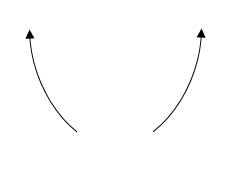
\includegraphics[width=0.3\textwidth]{../Figures/polyEndBehaviorCA.png}
\end{center}\begin{enumerate}[label=\Alph*.]
\begin{multicols}{2}
\item 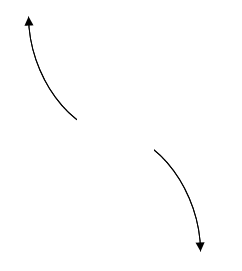
\includegraphics[width = 0.3\textwidth]{../Figures/polyEndBehaviorAA.png}
\item 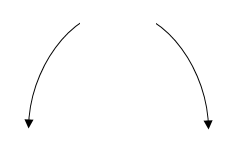
\includegraphics[width = 0.3\textwidth]{../Figures/polyEndBehaviorBA.png}
\item 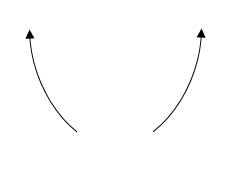
\includegraphics[width = 0.3\textwidth]{../Figures/polyEndBehaviorCA.png}
\item 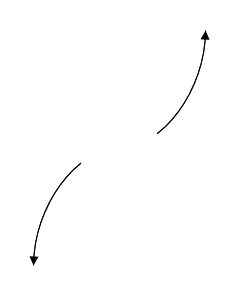
\includegraphics[width = 0.3\textwidth]{../Figures/polyEndBehaviorDA.png}
\end{multicols}\item None of the above.\end{enumerate}
\textbf{General Comment:} Remember that end behavior is determined by the leading coefficient AND whether the \textbf{sum} of the multiplicities is positive or negative.
}
\litem{
Describe the zero behavior of the zero $x = 3$ of the polynomial below.
\[ f(x) = -4(x - 8)^{5}(x + 8)^{4}(x - 3)^{8}(x + 3)^{5} \]
The solution is the graph below, which is option C.
\begin{center}
    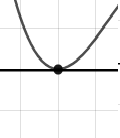
\includegraphics[width=0.3\textwidth]{../Figures/polyZeroBehaviorCopyCA.png}
\end{center}\begin{enumerate}[label=\Alph*.]
\begin{multicols}{2}
\item 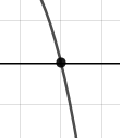
\includegraphics[width = 0.3\textwidth]{../Figures/polyZeroBehaviorCopyAA.png}
\item 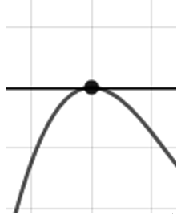
\includegraphics[width = 0.3\textwidth]{../Figures/polyZeroBehaviorCopyBA.png}
\item 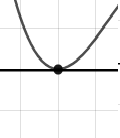
\includegraphics[width = 0.3\textwidth]{../Figures/polyZeroBehaviorCopyCA.png}
\item 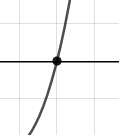
\includegraphics[width = 0.3\textwidth]{../Figures/polyZeroBehaviorCopyDA.png}
\end{multicols}\item None of the above.\end{enumerate}
\textbf{General Comment:} You will need to sketch the entire graph, then zoom in on the zero the question asks about.
}
\litem{
Describe the zero behavior of the zero $x = -3$ of the polynomial below.
\[ f(x) = 9(x + 3)^{5}(x - 3)^{10}(x - 6)^{8}(x + 6)^{11} \]
The solution is the graph below, which is option D.
\begin{center}
    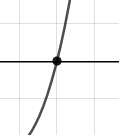
\includegraphics[width=0.3\textwidth]{../Figures/polyZeroBehaviorDA.png}
\end{center}\begin{enumerate}[label=\Alph*.]
\begin{multicols}{2}
\item 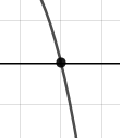
\includegraphics[width = 0.3\textwidth]{../Figures/polyZeroBehaviorAA.png}
\item 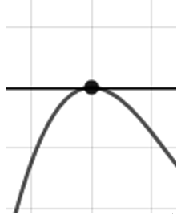
\includegraphics[width = 0.3\textwidth]{../Figures/polyZeroBehaviorBA.png}
\item 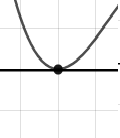
\includegraphics[width = 0.3\textwidth]{../Figures/polyZeroBehaviorCA.png}
\item 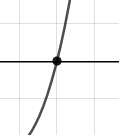
\includegraphics[width = 0.3\textwidth]{../Figures/polyZeroBehaviorDA.png}
\end{multicols}\item None of the above.\end{enumerate}
\textbf{General Comment:} You will need to sketch the entire graph, then zoom in on the zero the question asks about.
}
\litem{
Construct the lowest-degree polynomial given the zeros below. Then, choose the intervals that contain the coefficients of the polynomial in the form $x^3+bx^2+cx+d$.
\[ 5 - 2 i \text{ and } -1 \]
The solution is \( x^{3} -9 x^{2} +19 x + 29 \), which is option C.\begin{enumerate}[label=\Alph*.]
\item \( b \in [-1, 7], c \in [0, 8], \text{ and } d \in [2, 6] \)

$x^{3} + x^{2} +3 x + 2$, which corresponds to multiplying out $(x + 2)(x + 1)$.
\item \( b \in [-1, 7], c \in [-9, -3], \text{ and } d \in [-5, -2] \)

$x^{3} + x^{2} -4 x -5$, which corresponds to multiplying out $(x -5)(x + 1)$.
\item \( b \in [-9, -6], c \in [15, 20], \text{ and } d \in [25, 36] \)

* $x^{3} -9 x^{2} +19 x + 29$, which is the correct option.
\item \( b \in [6, 16], c \in [15, 20], \text{ and } d \in [-30, -27] \)

$x^{3} +9 x^{2} +19 x -29$, which corresponds to multiplying out $(x-(5 - 2 i))(x-(5 + 2 i))(x -1)$.
\item \( \text{None of the above.} \)

This corresponds to making an unanticipated error or not understanding how to use nonreal complex numbers to create the lowest-degree polynomial. If you chose this and are not sure what you did wrong, please contact the coordinator for help.
\end{enumerate}

\textbf{General Comment:} Remember that the conjugate of $a+bi$ is $a-bi$. Since these zeros always come in pairs, we need to multiply out $(x-(5 - 2 i))(x-(5 + 2 i))(x-(-1))$.
}
\litem{
Which of the following equations \textit{could} be of the graph presented below?

\begin{center}
    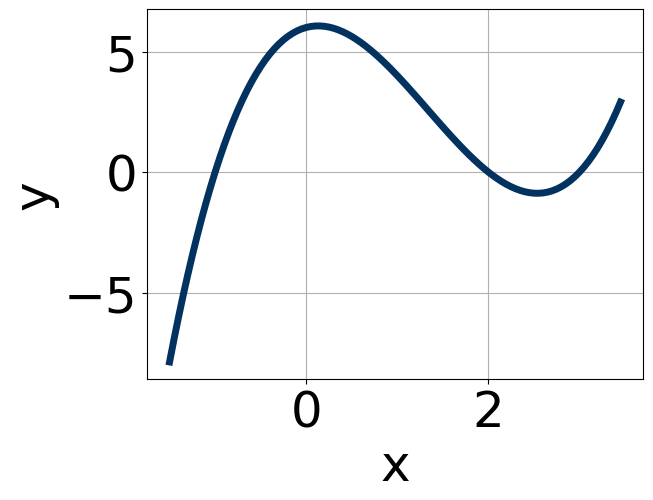
\includegraphics[width=0.5\textwidth]{../Figures/polyGraphToFunctionCopyA.png}
\end{center}



The solution is \( 10(x - 3)^{7} (x - 2)^{7} (x + 1)^{11} \), which is option E.\begin{enumerate}[label=\Alph*.]
\item \( -14(x - 3)^{8} (x - 2)^{9} (x + 1)^{11} \)

The factor $(x - 3)$ should have an odd power and the leading coefficient should be the opposite sign.
\item \( 18(x - 3)^{6} (x - 2)^{7} (x + 1)^{7} \)

The factor $3$ should have been an odd power.
\item \( 4(x - 3)^{4} (x - 2)^{8} (x + 1)^{7} \)

The factors $3$ and $2$ have have been odd power.
\item \( -12(x - 3)^{5} (x - 2)^{7} (x + 1)^{11} \)

This corresponds to the leading coefficient being the opposite value than it should be.
\item \( 10(x - 3)^{7} (x - 2)^{7} (x + 1)^{11} \)

* This is the correct option.
\end{enumerate}

\textbf{General Comment:} General Comments: Draw the x-axis to determine which zeros are touching (and so have even multiplicity) or cross (and have odd multiplicity).
}
\litem{
Construct the lowest-degree polynomial given the zeros below. Then, choose the intervals that contain the coefficients of the polynomial in the form $ax^3+bx^2+cx+d$.
\[ \frac{6}{5}, \frac{-7}{4}, \text{ and } \frac{-3}{4} \]
The solution is \( 80x^{3} +104 x^{2} -135 x -126 \), which is option E.\begin{enumerate}[label=\Alph*.]
\item \( a \in [75, 83], b \in [104, 107], c \in [-137, -125], \text{ and } d \in [122, 127] \)

$80x^{3} +104 x^{2} -135 x + 126$, which corresponds to multiplying everything correctly except the constant term.
\item \( a \in [75, 83], b \in [13, 24], c \in [-203, -197], \text{ and } d \in [-128, -119] \)

$80x^{3} +16 x^{2} -201 x -126$, which corresponds to multiplying out $(5x + 5)(4x + 4)(4x -4)$.
\item \( a \in [75, 83], b \in [296, 299], c \in [341, 351], \text{ and } d \in [122, 127] \)

$80x^{3} +296 x^{2} +345 x + 126$, which corresponds to multiplying out $(5x + 5)(4x -4)(4x -4)$.
\item \( a \in [75, 83], b \in [-104, -99], c \in [-137, -125], \text{ and } d \in [122, 127] \)

$80x^{3} -104 x^{2} -135 x + 126$, which corresponds to multiplying out $(5x + 6)(4x -7)(4x -3)$.
\item \( a \in [75, 83], b \in [104, 107], c \in [-137, -125], \text{ and } d \in [-128, -119] \)

* $80x^{3} +104 x^{2} -135 x -126$, which is the correct option.
\end{enumerate}

\textbf{General Comment:} To construct the lowest-degree polynomial, you want to multiply out $(5x -6)(4x + 7)(4x + 3)$
}
\litem{
Construct the lowest-degree polynomial given the zeros below. Then, choose the intervals that contain the coefficients of the polynomial in the form $x^3+bx^2+cx+d$.
\[ 3 + 5 i \text{ and } 4 \]
The solution is \( x^{3} -10 x^{2} +58 x -136 \), which is option C.\begin{enumerate}[label=\Alph*.]
\item \( b \in [-4, 4], c \in [-11, -8], \text{ and } d \in [19, 24] \)

$x^{3} + x^{2} -9 x + 20$, which corresponds to multiplying out $(x -5)(x -4)$.
\item \( b \in [-4, 4], c \in [-7, -4], \text{ and } d \in [6, 15] \)

$x^{3} + x^{2} -7 x + 12$, which corresponds to multiplying out $(x -3)(x -4)$.
\item \( b \in [-11, -4], c \in [54, 66], \text{ and } d \in [-137, -132] \)

* $x^{3} -10 x^{2} +58 x -136$, which is the correct option.
\item \( b \in [10, 13], c \in [54, 66], \text{ and } d \in [135, 138] \)

$x^{3} +10 x^{2} +58 x + 136$, which corresponds to multiplying out $(x-(3 + 5 i))(x-(3 - 5 i))(x + 4)$.
\item \( \text{None of the above.} \)

This corresponds to making an unanticipated error or not understanding how to use nonreal complex numbers to create the lowest-degree polynomial. If you chose this and are not sure what you did wrong, please contact the coordinator for help.
\end{enumerate}

\textbf{General Comment:} Remember that the conjugate of $a+bi$ is $a-bi$. Since these zeros always come in pairs, we need to multiply out $(x-(3 + 5 i))(x-(3 - 5 i))(x-(4))$.
}
\litem{
Describe the end behavior of the polynomial below.
\[ f(x) = 6(x + 9)^{2}(x - 9)^{3}(x + 6)^{3}(x - 6)^{3} \]
The solution is the graph below, which is option D.
\begin{center}
    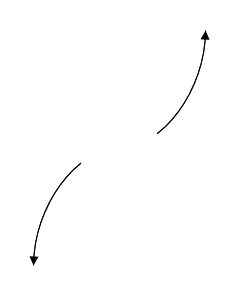
\includegraphics[width=0.3\textwidth]{../Figures/polyEndBehaviorCopyDA.png}
\end{center}\begin{enumerate}[label=\Alph*.]
\begin{multicols}{2}
\item 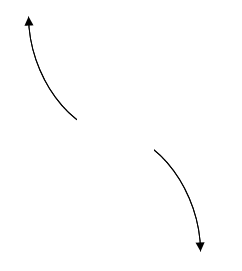
\includegraphics[width = 0.3\textwidth]{../Figures/polyEndBehaviorCopyAA.png}
\item 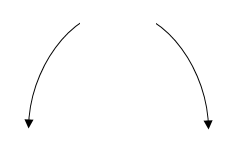
\includegraphics[width = 0.3\textwidth]{../Figures/polyEndBehaviorCopyBA.png}
\item 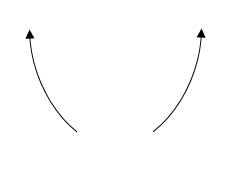
\includegraphics[width = 0.3\textwidth]{../Figures/polyEndBehaviorCopyCA.png}
\item 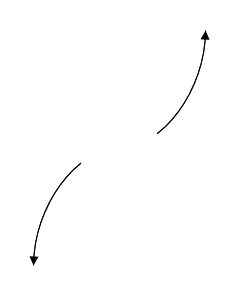
\includegraphics[width = 0.3\textwidth]{../Figures/polyEndBehaviorCopyDA.png}
\end{multicols}\item None of the above.\end{enumerate}
\textbf{General Comment:} Remember that end behavior is determined by the leading coefficient AND whether the \textbf{sum} of the multiplicities is positive or negative.
}
\litem{
Construct the lowest-degree polynomial given the zeros below. Then, choose the intervals that contain the coefficients of the polynomial in the form $ax^3+bx^2+cx+d$.
\[ \frac{-1}{4}, \frac{-1}{5}, \text{ and } 5 \]
The solution is \( 20x^{3} -91 x^{2} -44 x -5 \), which is option C.\begin{enumerate}[label=\Alph*.]
\item \( a \in [15, 26], b \in [-94, -89], c \in [-48, -42], \text{ and } d \in [0, 6] \)

$20x^{3} -91 x^{2} -44 x + 5$, which corresponds to multiplying everything correctly except the constant term.
\item \( a \in [15, 26], b \in [-101, -98], c \in [3, 5], \text{ and } d \in [0, 6] \)

$20x^{3} -101 x^{2} +4 x + 5$, which corresponds to multiplying out $(4x + 4)(5x -5)(x -1)$.
\item \( a \in [15, 26], b \in [-94, -89], c \in [-48, -42], \text{ and } d \in [-6, 2] \)

* $20x^{3} -91 x^{2} -44 x -5$, which is the correct option.
\item \( a \in [15, 26], b \in [90, 92], c \in [-48, -42], \text{ and } d \in [0, 6] \)

$20x^{3} +91 x^{2} -44 x + 5$, which corresponds to multiplying out $(4x -1)(5x -1)(x + 5)$.
\item \( a \in [15, 26], b \in [-109, -104], c \in [45, 48], \text{ and } d \in [-6, 2] \)

$20x^{3} -109 x^{2} +46 x -5$, which corresponds to multiplying out $(4x + 4)(5x + 5)(x -1)$.
\end{enumerate}

\textbf{General Comment:} To construct the lowest-degree polynomial, you want to multiply out $(4x + 1)(5x + 1)(x -5)$
}
\litem{
Which of the following equations \textit{could} be of the graph presented below?

\begin{center}
    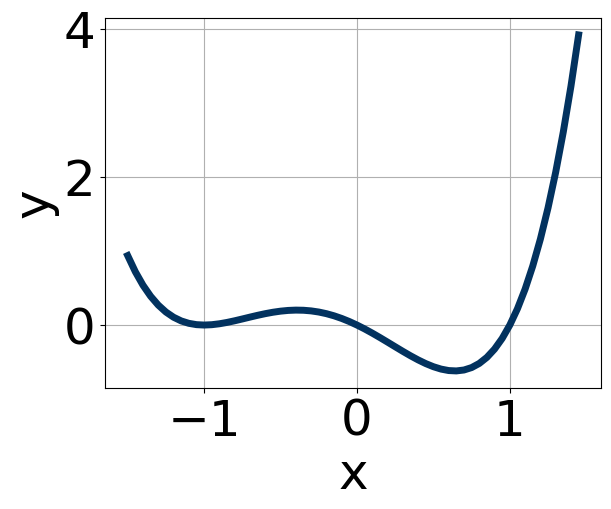
\includegraphics[width=0.5\textwidth]{../Figures/polyGraphToFunctionA.png}
\end{center}



The solution is \( -5x^{10} (x - 1)^{8} (x + 2)^{7} \), which is option A.\begin{enumerate}[label=\Alph*.]
\item \( -5x^{10} (x - 1)^{8} (x + 2)^{7} \)

* This is the correct option.
\item \( -9x^{5} (x - 1)^{4} (x + 2)^{4} \)

The factor $x$ should have an even power and the factor $(x + 2)$ should have an odd power.
\item \( -8x^{7} (x - 1)^{10} (x + 2)^{11} \)

The factor $x$ should have an even power.
\item \( 17x^{10} (x - 1)^{6} (x + 2)^{6} \)

The factor $(x + 2)$ should have an odd power and the leading coefficient should be the opposite sign.
\item \( 4x^{4} (x - 1)^{10} (x + 2)^{9} \)

This corresponds to the leading coefficient being the opposite value than it should be.
\end{enumerate}

\textbf{General Comment:} General Comments: Draw the x-axis to determine which zeros are touching (and so have even multiplicity) or cross (and have odd multiplicity).
}
\end{enumerate}

\end{document}